\documentclass[12pt]{article}
\usepackage{fullpage,enumitem,amsmath,amssymb,graphicx}
\usepackage{graphicx} % This is a package for including graphics in your solution.
\usepackage{listings}
\usepackage[final]{pdfpages}

\begin{document}

\begin{center}
{\Large CS168 Spring Assignment 5}

\begin{tabular}{rl}
SUNet ID(s): 05794739 & \\
Name(s): & Luis A. Perez \\
Collaborators: &
\end{tabular}
\end{center}

By turning in this assignment, I agree by the Stanford honor code and declare
that all of this is my own work.

\section*{Part 1}

\begin{enumerate}[label=(\alph*)]
  \item See Appendix for code. 
  \item See Figure \ref{fig:singular_values} for the plot. From the plot we can see
    that the singular values decay relatively quickly. This implies that there exists a fairly low-rank approximation of $M$.

    \begin{figure}[!ht]
      \centering
      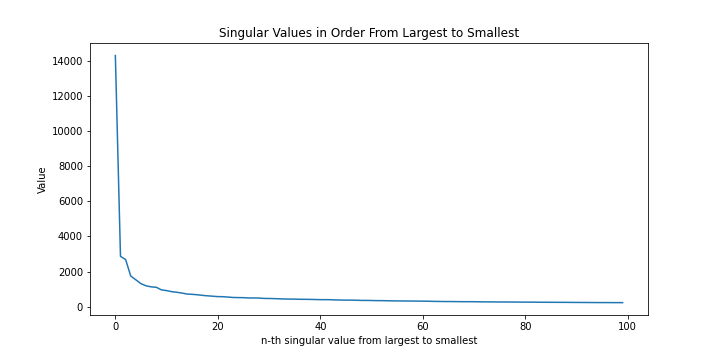
\includegraphics[scale=0.5]{figures/singular_values.png}
      \caption{Singular values of $\tilde{M}$ from largest to smallest}
      \label{fig:singular_values}
    \end{figure}
  \item
    A few interesting vectors. We have $v_3$ which gives the following:
    \begin{verbatim}
Top 10 Words
['michael', 'thomas', 'george', 'jr', 'william', 'robert', 'david', 'james', 'john', 'born']
Bottom 10 Words
['specific', 'any', 'data', 'provide', 'these', 'certain', 'different', 'systems', 'its', 'use']
    \end{verbatim}
    This appears to be a vector encoding the concept of a `name' or `title' (maybe also person)?

    Also $v_6$
    \begin{verbatim}
Top 10 Words
['electronic', 'web', 'online', 'research', 'computer', 'engineering', 'technology', 'software', 'science', 'digital']
Bottom 10 Words
['troops', 'him', 'killed', 'soldiers', 'they', 'them', 'were', 'had', 'emperor', 'attacked']
    \end{verbatim}
    This appears to encode the concept of `technology'.

    Also $v_8$:
    \begin{verbatim}
Top 10 Words
['entered', 'became', 'came', 'moved', 'served', 'joined', 'led', 'brought', 'gave', 'took']
Bottom 10 Words
['him', 'them', 'it', 'himself', 'her', 'students', 'who', 'government', 'people', 'players']
    \end{verbatim}
    Which appears to encode the concept of `movement`.

    Also $v_{15}$:
    \begin{verbatim}
Top 10 Words
['subsequent', 'scenes', 'combat', 'completed', 'training', 'artillery', 'battle', 'brief', 'naval', 'squadron']
Bottom 10 Words
['brazil', 'products', 'food', 'income', 'municipality', 'born', 'population', 'name', 'milk', 'province']
    \end{verbatim}
    This appears to encode the concept of military units.

    And lastly, $v_{22}$:
    \begin{verbatim}
Top 10 Words
['institute', 'band', 'records', 'remix', 'and', 'university', 'vol', 'cd', 'album', 'lp']
Bottom 10 Words
['characters', 'television', 'location', 'character', 'actor', 'channel', 'bbc', 'plot', 'journalist', 'actress']   
    \end{verbatim}
    Which appears to encode musical storage devices.

    The reason why not all vectors have easy to intepret semantics is because they're capturing the directions of highest variability, and as such might capture fairly complex semantic meaning that are difficult to interpret.
  
  \item
    \begin{enumerate}[label=\roman*]
      \item
        The plot is presented in Figure \ref{fig:projection_ont_femaleness}. We observe that the more feminise a word is, the closer the projection gets to 1.0.

        \begin{figure}[!ht]
          \centering
          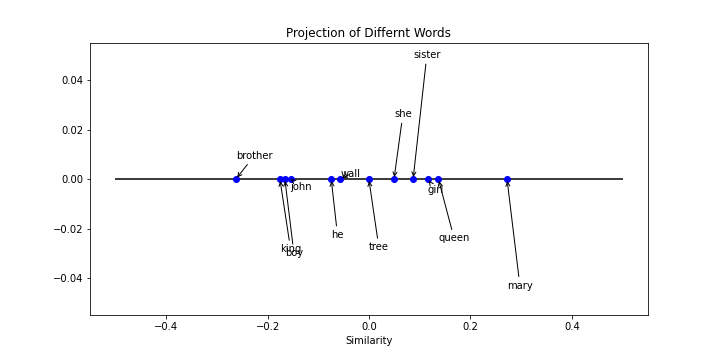
\includegraphics[scale=0.5]{figures/projection_onto_femaleness.png}
          \caption{Projection of multiple words onto $v_2 - v_1$ where $v_2$ is the embedding vector corresponding to woman and $v_1$ is the one corresponding to man.}
          \label{fig:projection_ont_femaleness}
        \end{figure}
      \item
       The plot is presented in Figure \ref{fig:projection_ont_femaleness_2}. We observe that certain words (which should have little association with femininity) are, and other words are counter associated.

       This is likely due to bias in our training data -- that is to say, female words appeared frequently with words such as `nurse' and `teacher' while far less frequently with words such as `engineer' and `science'. This has led to the model capturing these biased relation in its embeddings, which is bad since it is prejudiced against women in certain fields.

        \begin{figure}[!ht]
          \centering
          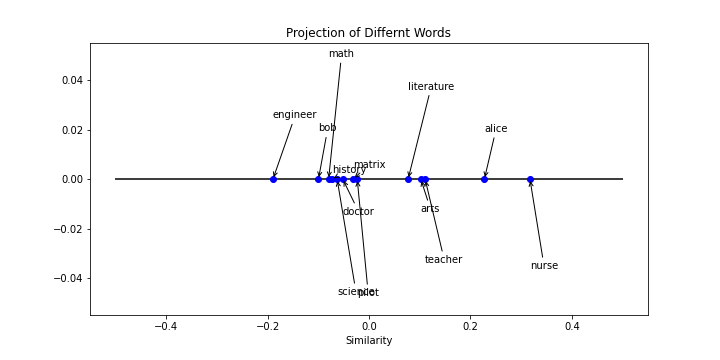
\includegraphics[scale=0.5]{figures/projection_ton_femaleness_2.png}
          \caption{Projection of multiple words onto $v_2 - v_1$ where $v_2$ is the embedding vector corresponding to woman and $v_1$ is the one corresponding to man.}
          \label{fig:projection_ont_femaleness_2}
        \end{figure}

      \item
        The model learns what's in the data -- this is no fault of the model. As such, one approach would be to modify the input data so as to remove any gender-related words, or make sure that their co-occurrences with other words are always equal.
    \end{enumerate}

    \item
      \begin{enumerate}[label=\roman*]
        \item The closest word to 'stanford' is 'harvard'.
        \item The accuracy on the analogy task is 31.15487914055506\%.

          The method got any analogies related to places basically wrong (eg, if it requires factual information, the model is not able to accurately incorporate). It also struggled with analogies related to familial relationships. Lastly, it also appeared to struggle with analogies related to parts of speech (grammar).
      \end{enumerate}
\end{enumerate}

\newpage
\section*{Part 2}

\begin{enumerate}[label=(\alph*)]
  \item
    The rank-1 approximation of the picture of the moon should be a grey-ish square (darker on the outside, closer to the moon color near the center) surrounded by complete darkness.

    The reason for this is we can imagine taking the average of each row of pixels. This becomes are vector which will simply be scaled (either by 0 where it is black) or some non-zero value when crossing the moon area. 

  \item The 150-rank approximation is seen in Figure \ref{fig:low_rank}.
    \begin{figure}[!ht]
      \centering
      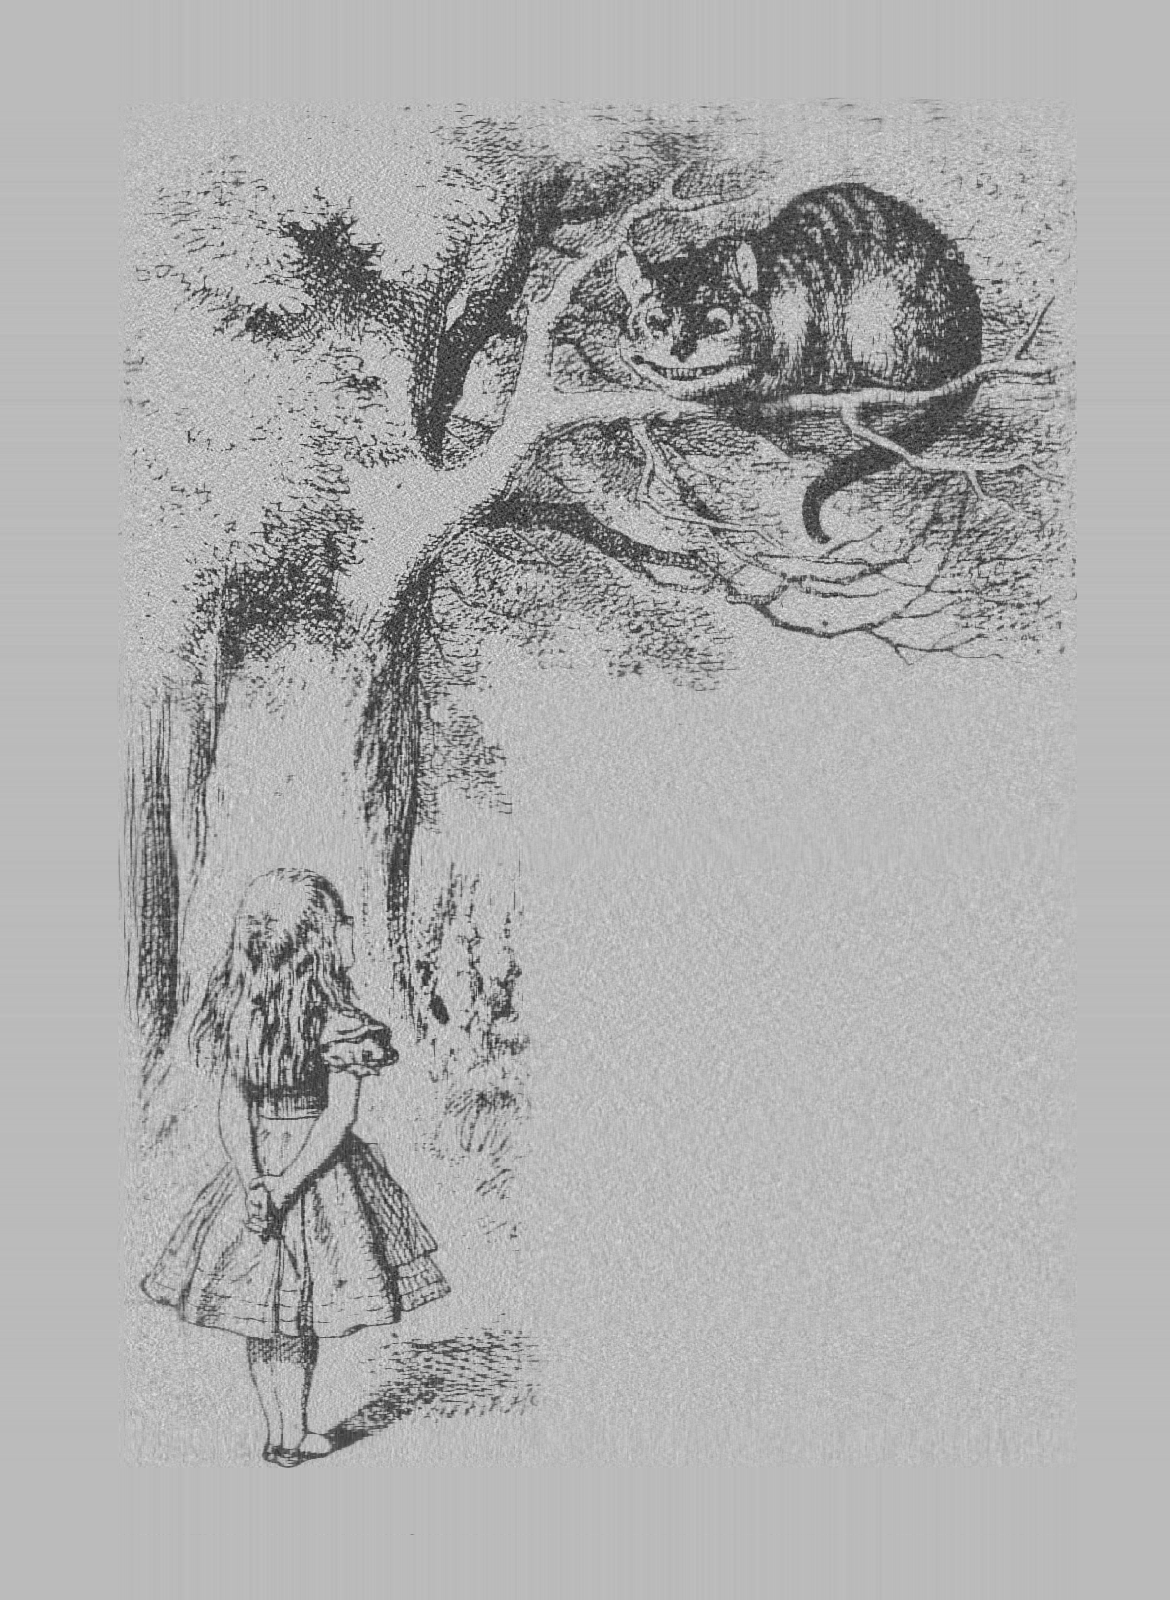
\includegraphics[scale=0.34]{figures/low_rank_alice.png}
      \caption{Compressed Image.}
      \label{fig:low_rank}    
    \end{figure}
  \item 1170 would recover the original image in its entirety.
  \item The approximation can be stored in at most 150x(1600 + 1170) = 415,500 bits of information. The original image (even if we don't store the 0 bits) requires 1,649,901 memory units. As such, in the worst case, we're saving 4x the amount of memory.
  \item Removing the haze in its entirety will requires having eigenvectors whose components are precisely 0 (so they aren't scaled up and down). Having these zero values essentially destroys significant amount of information. As such, these vectors aren't utilized until the very end when we compress the image less.
\end{enumerate}

\newpage
\section*{Appendix}
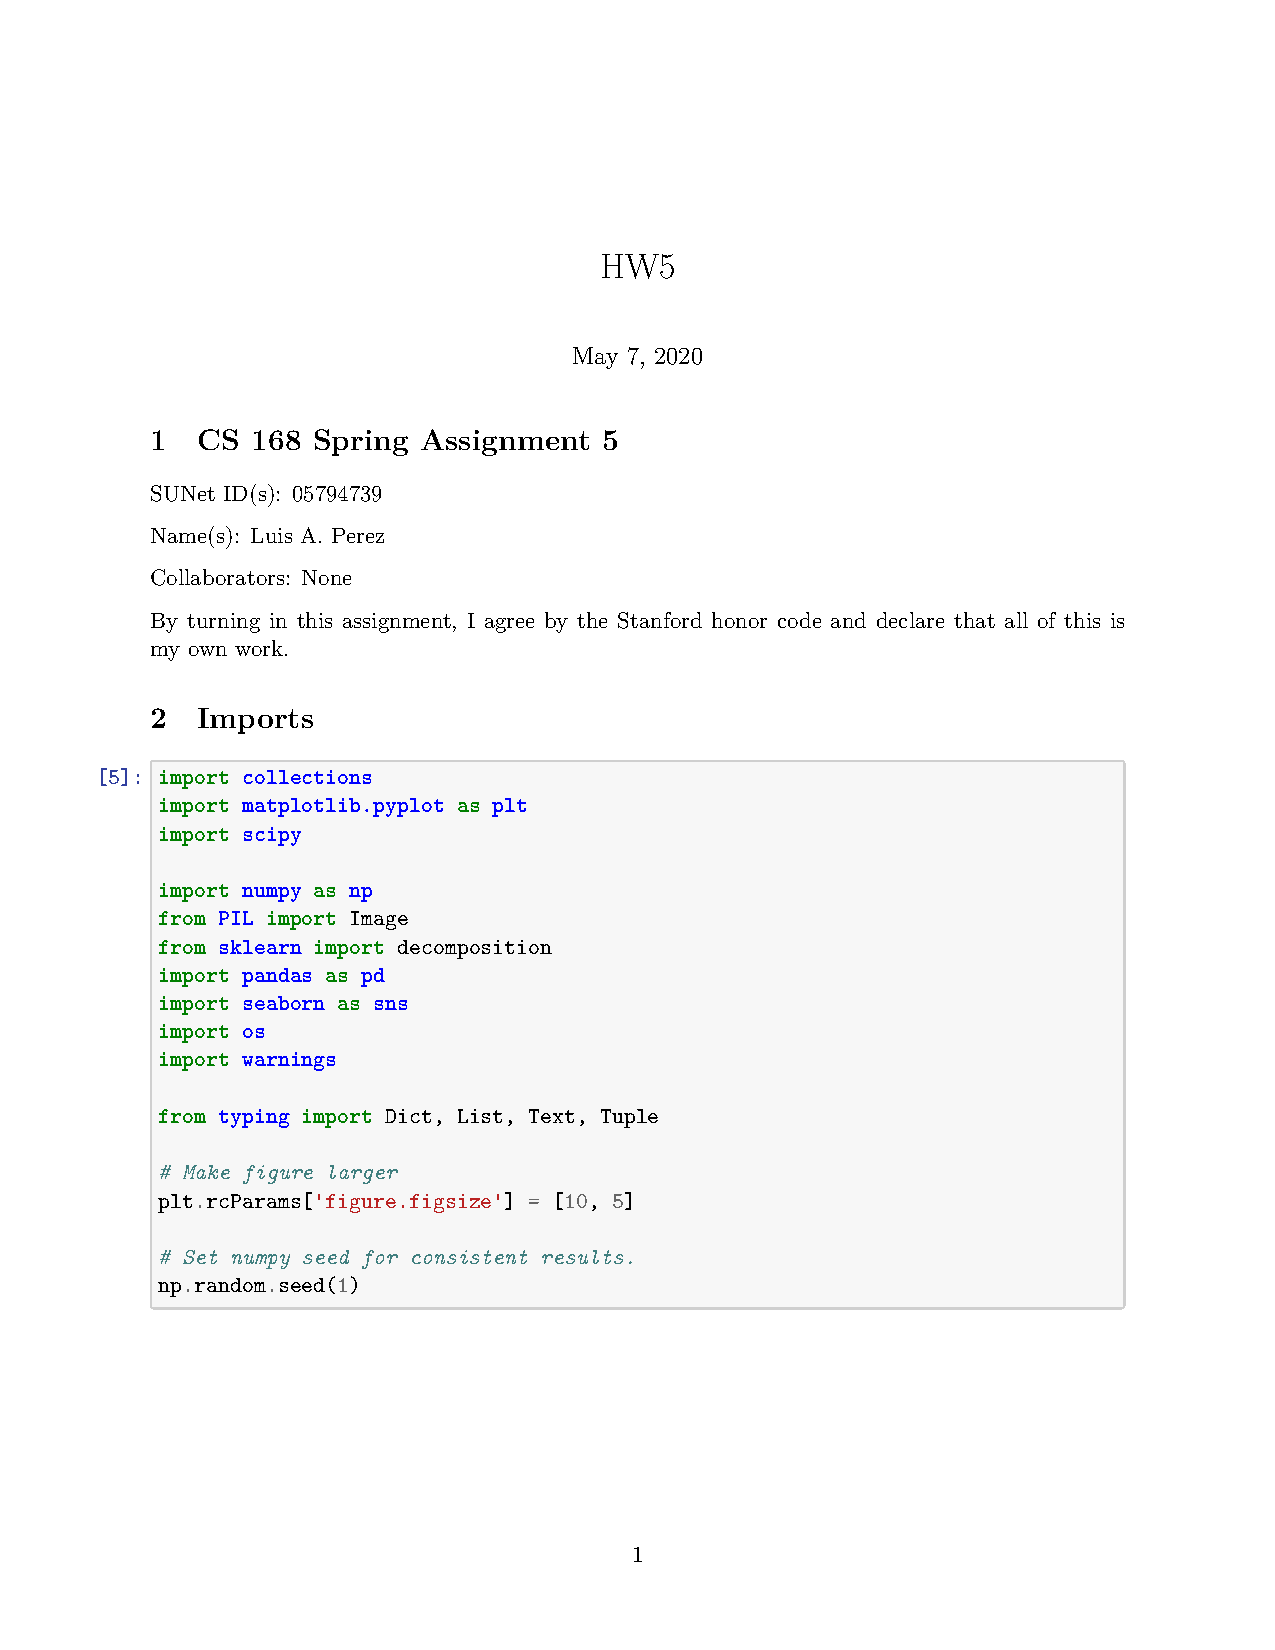
\includepdf[pages=-]{HW5}

\end{document}
